\section{TrainTicket}

Consider a microservices application called \texttt{TrainTicket} composed of 3 domain microservices (search, reserve, buy) and 1 additional microservice that acts as the API gateway. 
TrainTicket supports two basic operations invoked using the exposed RESTFul APIs:
\begin{enumerate}
    \item Search: /APIv1/search/{args}.
    \item Reserve: /APIv1/reserve/{args}.
\end{enumerate}
Requests (both search and reserve) are received and then dispatched by the API gateway.
In particular, the following high-level schema shows how requests propagate from the gateway to internal microservices.
Note that in this example reserve includes also the purchase of reserved items.
\begin{figure}[H]
    \centering
    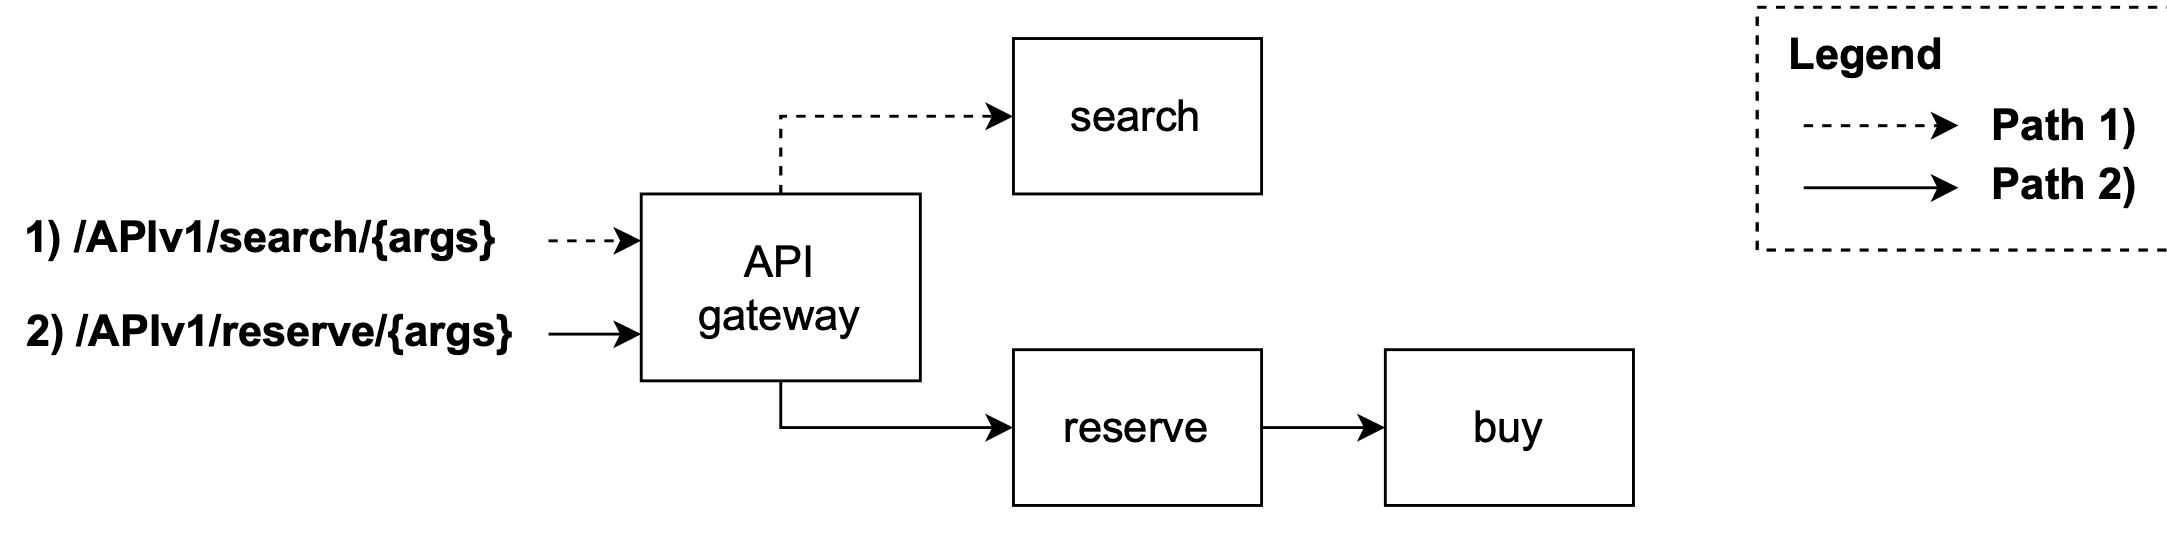
\includegraphics[width=0.5\linewidth]{images/hl.png}
\end{figure}
Microservices run in units deployed onto 2 different Virtual Machines, VM1 and VM2 as shown in the following UML deployment diagram.
The available VMs have Computational Resources (CRs) that can be allocated to run microservices.
Each VM has a maximum number of CRs and each microservice requires a certain number of CRs, according to the executed artifact. 
As shown in the schema, available CRs are as follows:
\begin{itemize}
    \item VM1: 20 CRs.
    \item VM2: 22 CRs.
\end{itemize}
\begin{figure}[H]
    \centering
    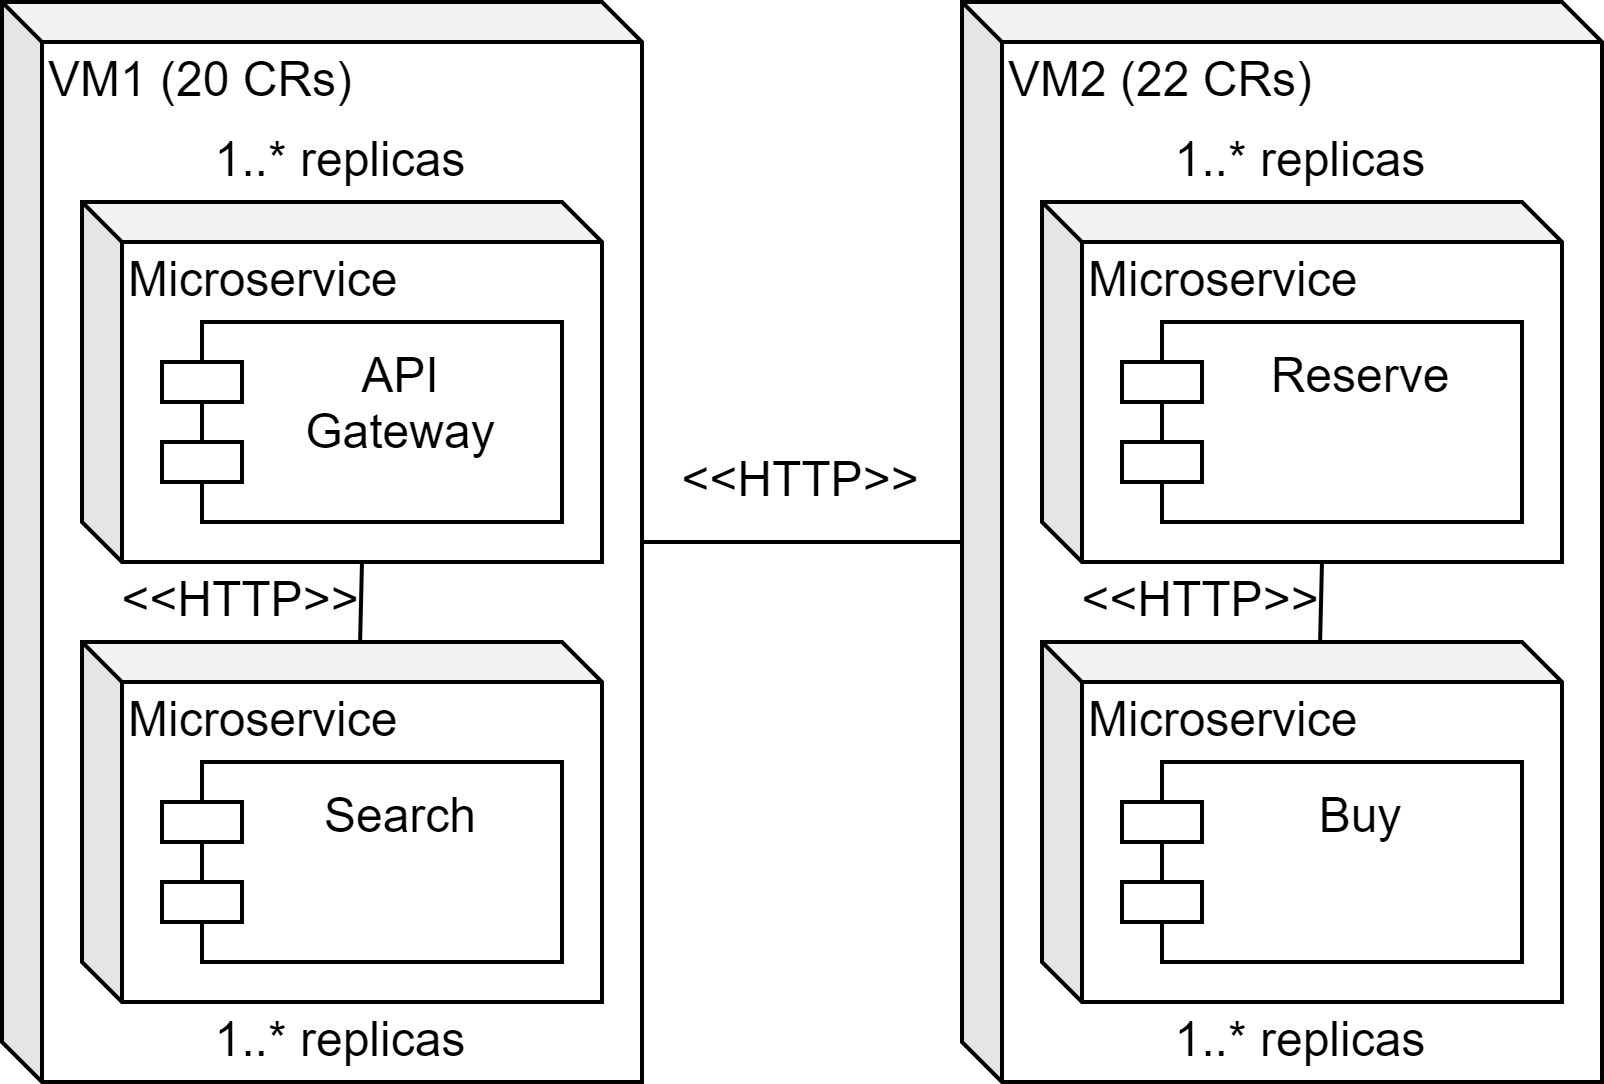
\includegraphics[width=0.75\linewidth]{images/hl1.png}
\end{figure}

The mapping between microservices and required CRs is as follows:
\begin{itemize}
    \item API gateway: 2 CRs.
    \item Search: 5 CRs.
    \item Reserve: 4 CRs.
    \item Buy: 5 CRs.
\end{itemize}
The deployment diagram shows that each microservice can be replicated to have redundant business-critical components. 
In the latter case, requests are directed to all the replicas rather than to an individual instance and the first answer received from a replica is returned to the caller, while the others are simply ignored. 
The number of replicas for each microservice shall be defined so that the following nonfunctional requirement is satisfied, and the deployment constraints defined in the deployment diagram and above are fulfilled.
We have also the following requirement: both search and reserve services exposed through API gateway shall have availability greater than or equal to 0.99. 
\begin{enumerate}
    \item Considering the constraints of the execution environment represented above, determine whether requirement R1 can be satisfied or not assuming the following availability estimates for each microservice: API gateway (0.99), search (0.98), reserve (0.95), and buy (0.91).
    \item Consider the problem of resource allocation taking into account the operational profile, that is, the behavior of the users. 
        Assume the following workload in terms of average number of concurrent users for each request:
        \begin{itemize}
            \item Search: 50 users. 
            \item Reserve: 90 users. 
        \end{itemize}
        Assume also that for reserve, only 20$\%$ of users complete the purchase at reservation time. This means that 20$\%$ of reserve requests get through and reach the buy microservice, while 80$\%$ of them terminate the execution without calling buy.
\end{enumerate}

\paragraph*{Solution}
\begin{enumerate}
    \item Considering the execution environment, we can derive the following equations constraining the number of replicas:
        \begin{itemize}
            \item $2x + 5y \leq 20$.
            \item $4u + 5z \leq 22$.
            \item $(1 - (1 - 0.99)x) \cdot (1 - (1 - 0.98)y) \geq 0.99$.
            \item $(1 - (1 - 0.99)x) \cdot (1 - (1 - 0.95)u) \cdot (1 - (1 - 0.91)z) \geq 0.99$. 
        \end{itemize}
        Where variables $x$, $y$, $u$, and $z$ represent the number of replicas for the microservices API gateway, search, reserve, and buy, respectively.
        The requirement R1 can be satisfied since there exists a valid assignment to variables that satisfies all constraints. 
        For instance: $x = 2$, $y = 2$, $u = 3$, and $z = 2$. 
    \item After a preliminary analysis, we realize that availability depends on the workload according to the following new estimates:
        \begin{table}[H]
            \centering
            \begin{tabular}{l|cc|}
            \cline{2-3}
            \multicolumn{1}{c|}{}                       & \textbf{Low workload} & \textbf{High workload} \\ \hline
            \multicolumn{1}{|l|}{\textbf{Microservice}} & \multicolumn{2}{c|}{\textit{Availability}}                                                     \\ \hline
            \multicolumn{1}{|l|}{\textbf{API gateway}}  & 0.99                                         & 0.98                                            \\
            \multicolumn{1}{|l|}{\textbf{Search}}       & 0.98                                         & 0.95                                            \\
            \multicolumn{1}{|l|}{\textbf{Reserve}}      & 0.95                                         & 0.93                                            \\
            \multicolumn{1}{|l|}{\textbf{Buy}}          & 0.91                                         & 0.90                                            \\ \hline
            \end{tabular}
        \end{table}
        The expected workload for each microservice is as follows:
        \begin{itemize}
            \item API gateway: 140 users (high). 
            \item Search: 50 users (low).
            \item Reserve: 90 users (high).
            \item Buy: 18 users (low).
        \end{itemize}
        The constraints extracted from requirement R1 become as follows:
        \[(1 - (1 - 0.98)x) \cdot (1 - (1 - 0.98)y) \geq 0.99\]
        \[(1 - (1 - 0.98)x) \cdot (1 - (1 - 0.93)u) \cdot (1 - (1 - 0.91)z) \geq 0.99\]
        An optimal resource allocation is represented by the assignment $x = 2$, $y = 2$, $u = 3$, and $z = 2$ that is again feasible according to environment constraints.
\end{enumerate}